\section{Results}
Table~\ref{tab:summary_metrics} reports the mean segmentation performance across the four benchmark histological images. The custom VeSpA pipeline achieved the highest mean Dice coefficient (\(0.7332\)) and IoU (\(0.5804\)). SAM ranked second with a mean Dice coefficient of \(0.2950\), while the pretrained YOLOv8 segmentation model achieved a mean Dice coefficient of \(0.0299\).

\begin{table}[htbp]
\centering
\caption{Mean performance metrics computed from \texttt{results/metrics/summary.csv}.}
\label{tab:summary_metrics}
\begin{tabular}{lcccc}
\hline
Model & Dice & IoU & Precision & Recall \\
\hline
VeSpA & 0.7332 & 0.5804 & 0.8171 & 0.6712 \\
SAM & 0.2950 & 0.1754 & 0.6509 & 0.1914 \\
YOLOv8-seg & 0.0299 & 0.0154 & 0.8567 & 0.0156 \\
\hline
\end{tabular}
\end{table}

Per-image results are shown in Table~\ref{tab:per_image_results}. VeSpA consistently outperformed the other methods on all four images, with Dice scores ranging from \(0.6776\) to \(0.7730\). SAM produced non-trivial but clearly inferior vessel masks, with Dice scores between \(0.1574\) and \(0.3424\). YOLOv8-seg returned sparse predictions and produced zero Dice on two of the four images.

\begin{table}[htbp]
\centering
\caption{Per-image Dice and IoU values extracted from \texttt{results/metrics/results.csv}.}
\label{tab:per_image_results}
\begin{tabular}{llcc}
\hline
Image & Model & Dice & IoU \\
\hline
ROI\_1 & VeSpA & 0.6776 & 0.5124 \\
ROI\_1 & SAM & 0.3385 & 0.2037 \\
ROI\_1 & YOLOv8-seg & 0.0700 & 0.0363 \\
ROI\_2 & VeSpA & 0.7100 & 0.5504 \\
ROI\_2 & SAM & 0.1574 & 0.0854 \\
ROI\_2 & YOLOv8-seg & 0.0494 & 0.0253 \\
ROI\_3 & VeSpA & 0.7730 & 0.6300 \\
ROI\_3 & SAM & 0.3424 & 0.2066 \\
ROI\_3 & YOLOv8-seg & 0.0000 & 0.0000 \\
ROI\_4 & VeSpA & 0.7722 & 0.6290 \\
ROI\_4 & SAM & 0.3415 & 0.2059 \\
ROI\_4 & YOLOv8-seg & 0.0000 & 0.0000 \\
\hline
\end{tabular}
\end{table}

Runtime measurements are summarized in Table~\ref{tab:runtime}. YOLOv8-seg was the fastest method with a mean runtime of \(0.59\) s per image, followed by VeSpA at \(2.57\) s per image. SAM was substantially slower, requiring \(23.35\) s per image under the current repository configuration.

\begin{table}[htbp]
\centering
\caption{Mean runtime per image from \texttt{results/metrics/runtime\_summary.csv}.}
\label{tab:runtime}
\begin{tabular}{lc}
\hline
Model & Runtime (s/image) \\
\hline
YOLOv8-seg & 0.59 \\
VeSpA & 2.57 \\
SAM & 23.35 \\
\hline
\end{tabular}
\end{table}

Figure~\ref{fig:dice_boxplot} visualizes the distribution of Dice scores, and Figure~\ref{fig:iou_bar} shows the mean IoU comparison. The plots confirm the ranking observed in the tabulated results. Qualitative overlays saved under \path{results/prediction/} are consistent with these metrics: VeSpA captures annotated vascular structures more completely, SAM identifies partial vessel structures while missing substantial foreground, and YOLOv8-seg produces highly conservative masks with low recall.

Figure~\ref{fig:roi1_example} provides a representative qualitative example for \texttt{ROI\_1}. Panel (a) shows the raw histological image. Panels (b)--(d) show the overlays generated by the benchmark for VeSpA, SAM, and YOLOv8-seg, respectively.

\begin{figure}[htbp]
\centering
\begin{subfigure}[t]{0.47\linewidth}
    \centering
    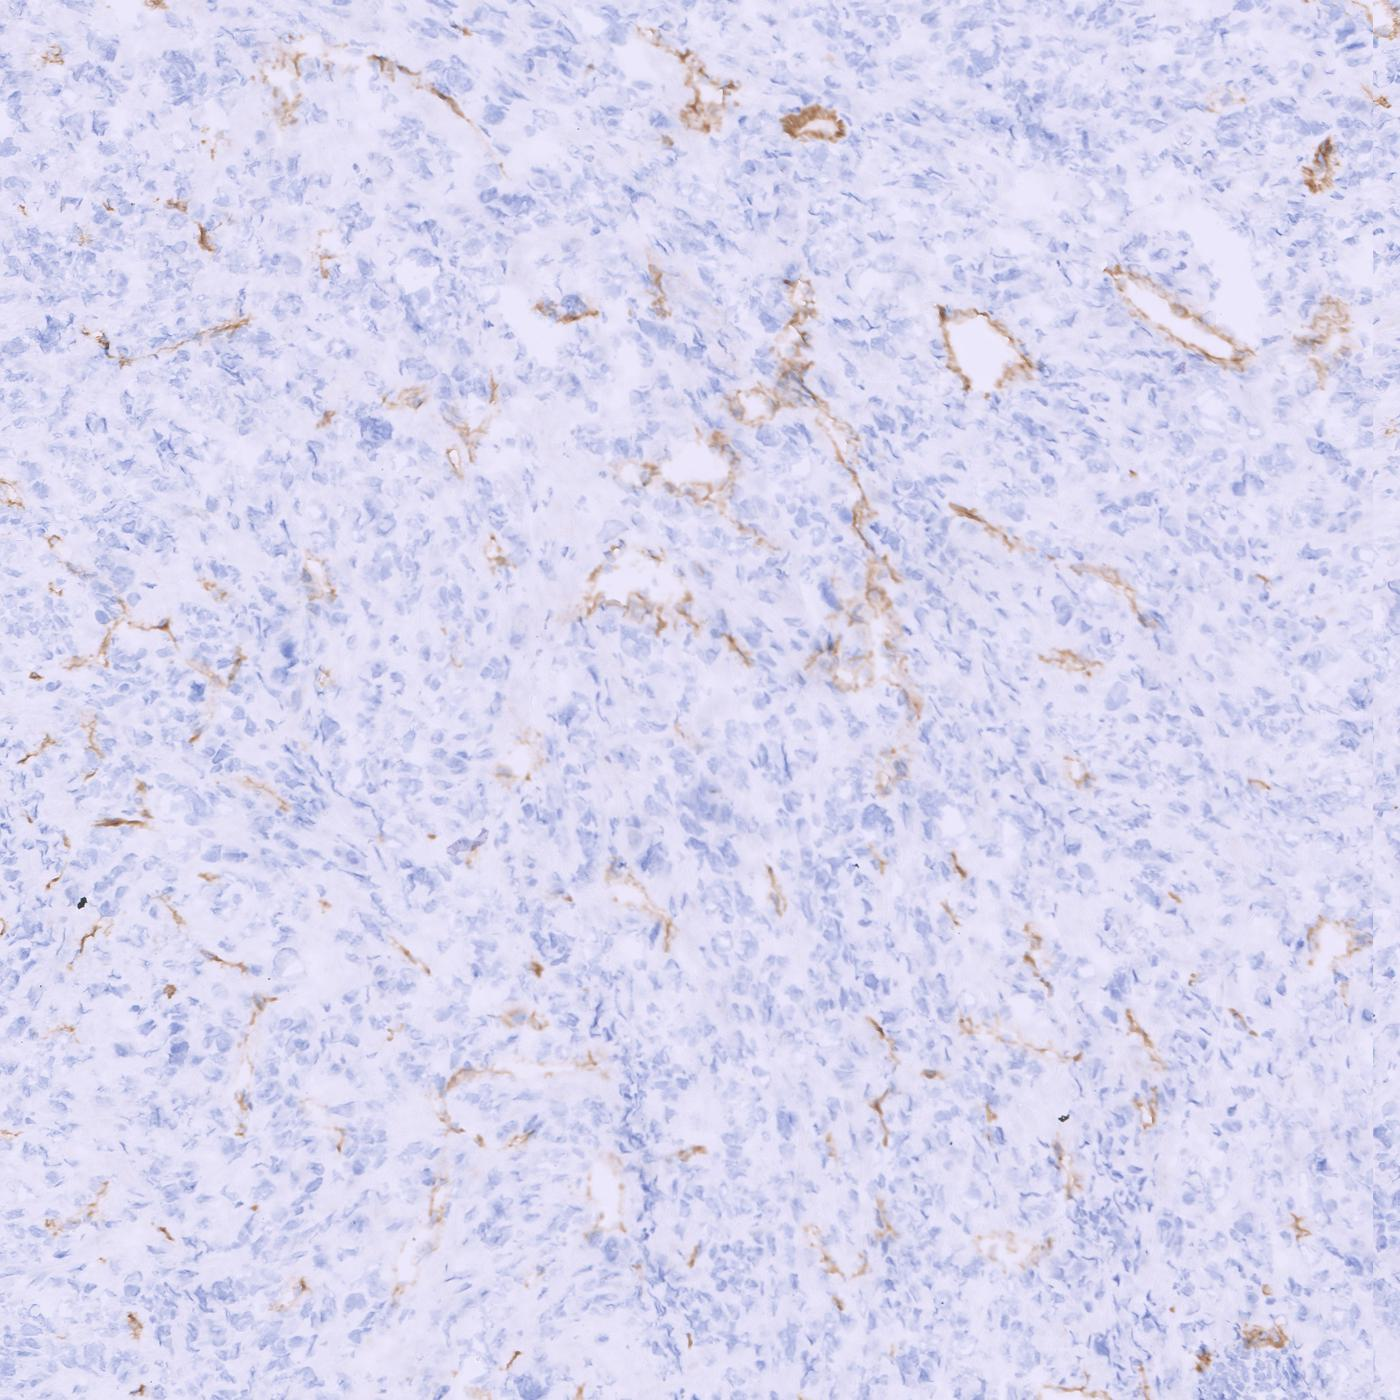
\includegraphics[width=\linewidth]{figures/ROI_1_raw_small.jpg}
    \caption{Raw image}
\end{subfigure}
\hfill
\begin{subfigure}[t]{0.47\linewidth}
    \centering
    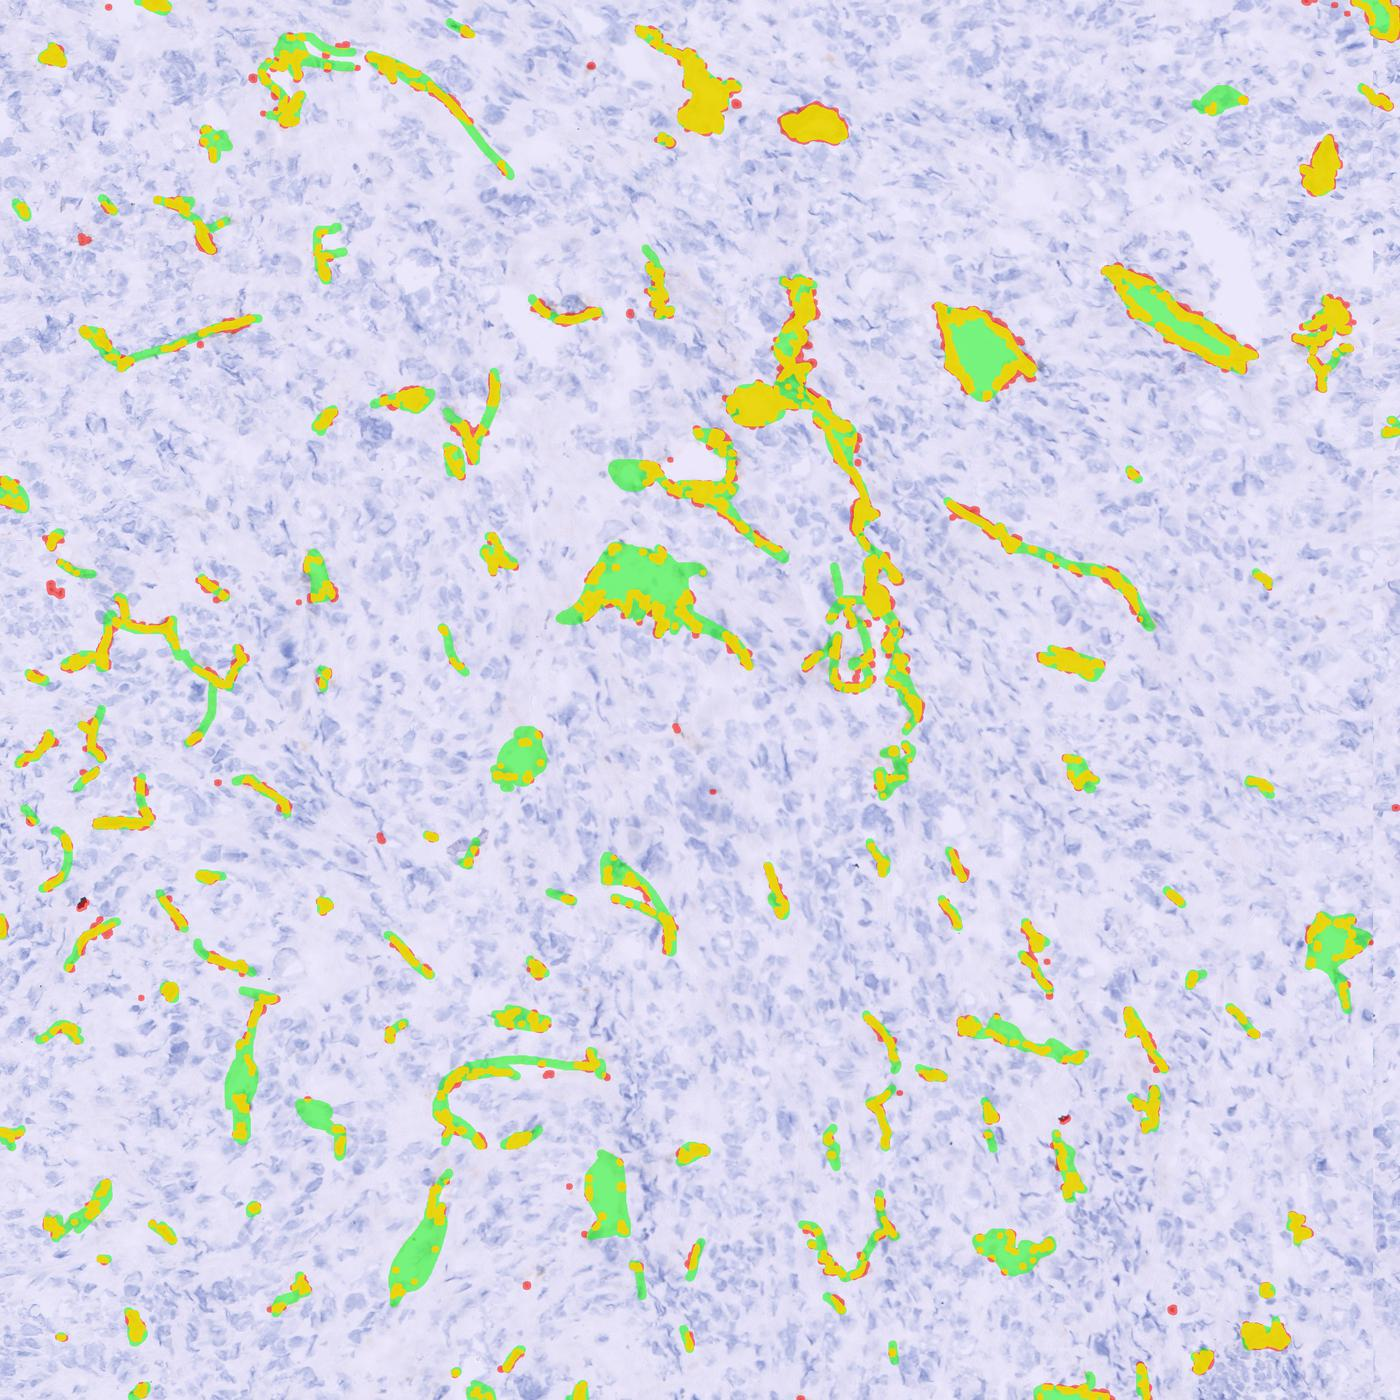
\includegraphics[width=\linewidth]{figures/ROI_1_vespa_overlay_small.jpg}
    \caption{VeSpA overlay}
\end{subfigure}

\vspace{0.6em}

\begin{subfigure}[t]{0.47\linewidth}
    \centering
    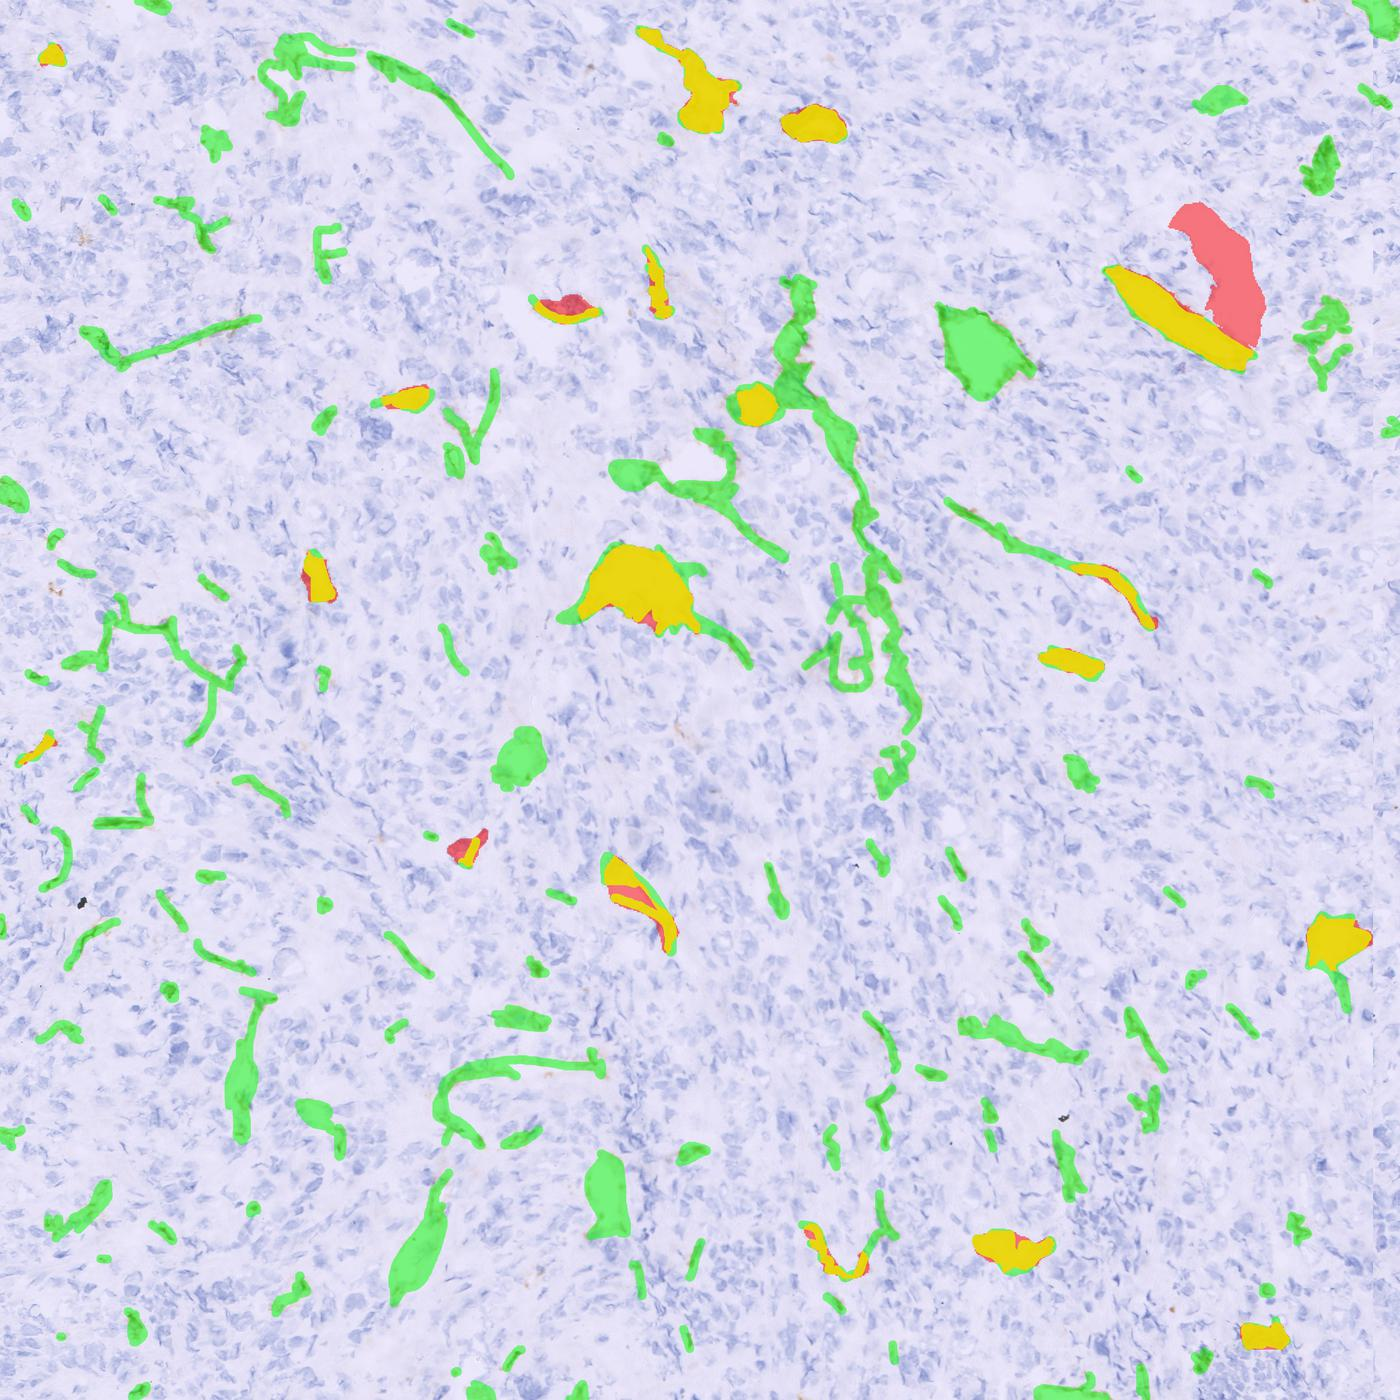
\includegraphics[width=\linewidth]{figures/ROI_1_sam_overlay_small.jpg}
    \caption{SAM overlay}
\end{subfigure}
\hfill
\begin{subfigure}[t]{0.47\linewidth}
    \centering
    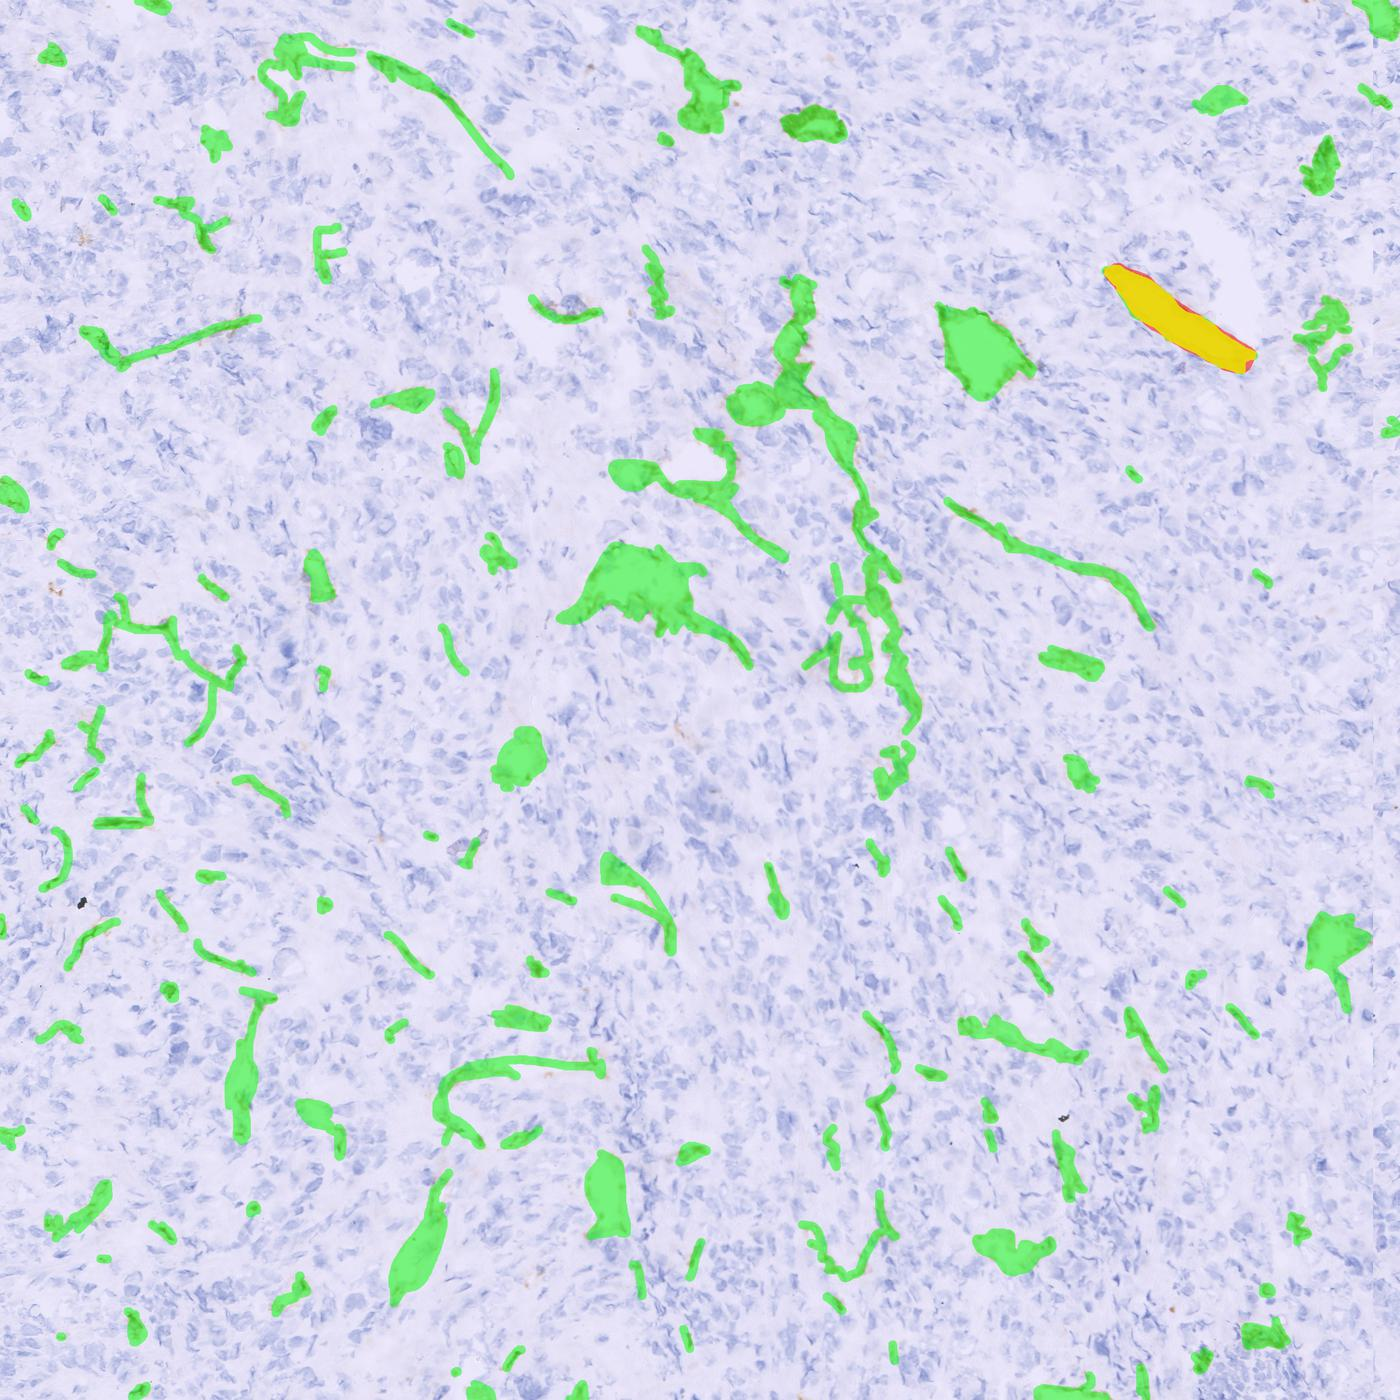
\includegraphics[width=\linewidth]{figures/ROI_1_yolo_overlay_small.jpg}
    \caption{YOLOv8-seg overlay}
\end{subfigure}
\caption{Representative qualitative example for \texttt{ROI\_1}. Panel (a) shows the raw histological image. Panels (b)--(d) show prediction overlays for VeSpA, SAM, and YOLOv8-seg. In the overlay visualizations, green denotes ground-truth vessel pixels, red denotes predicted vessel pixels, and yellow denotes spatial overlap between prediction and ground truth.}
\label{fig:roi1_example}
\end{figure}

\begin{figure}[htbp]
\centering
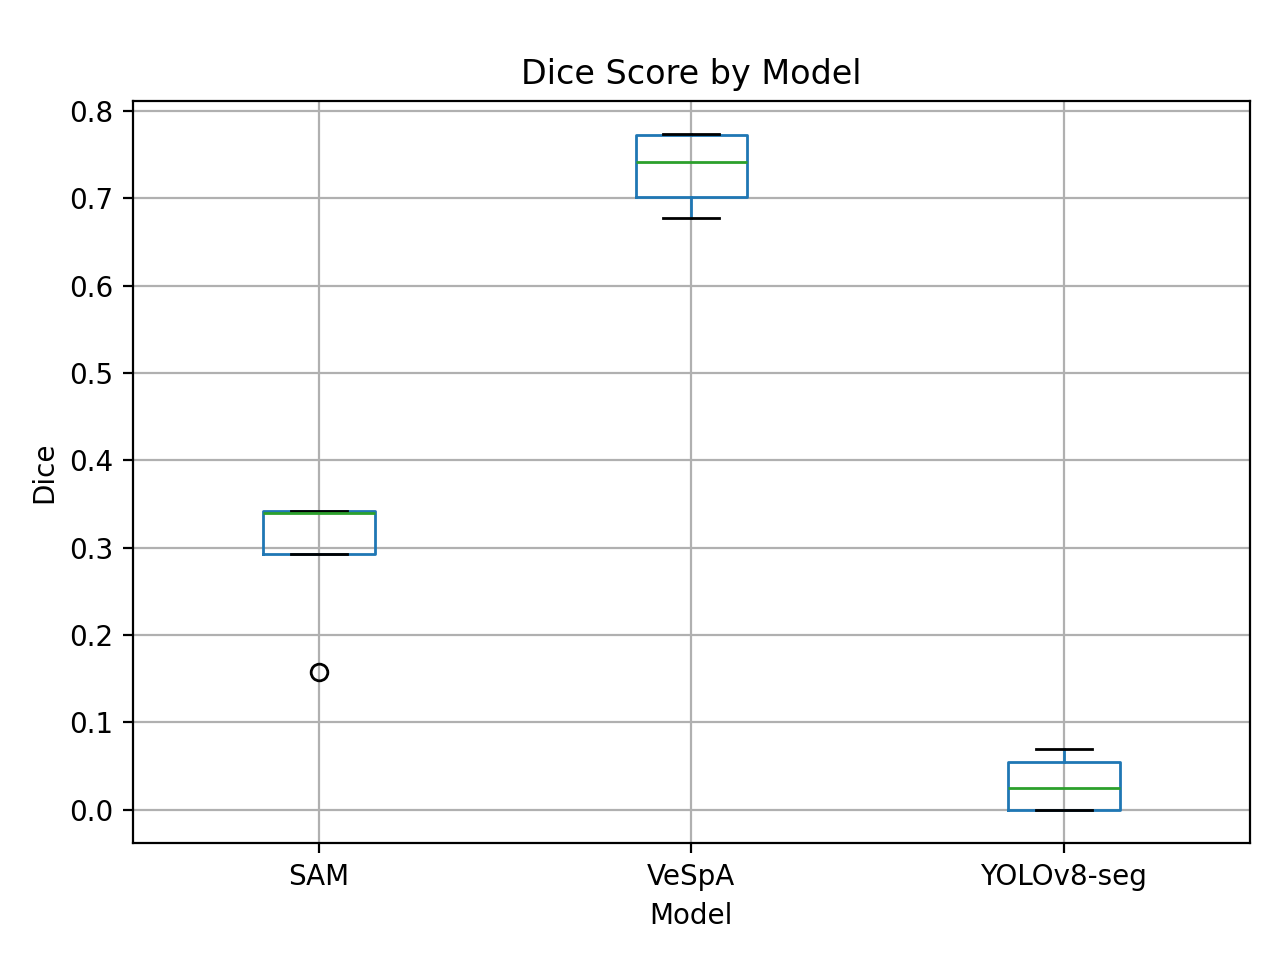
\includegraphics[width=0.7\linewidth]{../results/metrics/dice_boxplot.png}
\caption{Distribution of Dice scores across the four benchmark histological images.}
\label{fig:dice_boxplot}
\end{figure}

\begin{figure}[htbp]
\centering
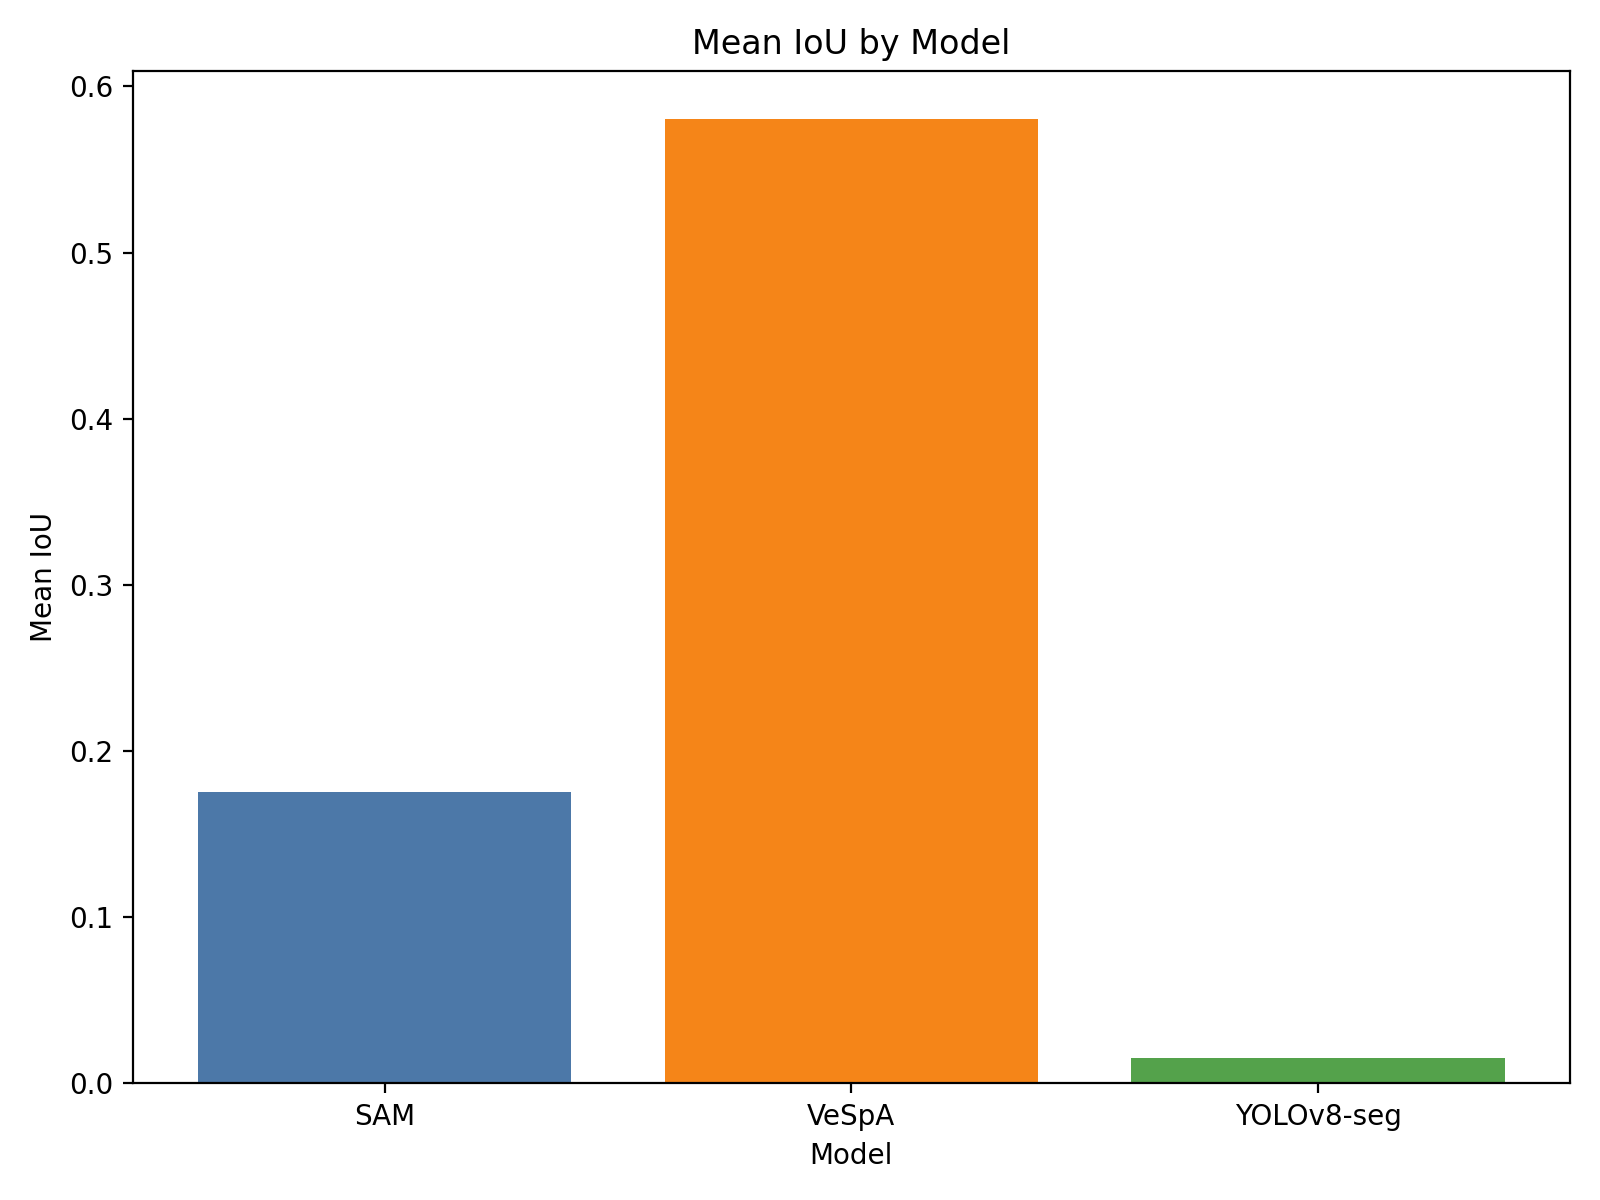
\includegraphics[width=0.7\linewidth]{../results/metrics/iou_comparison.png}
\caption{Mean IoU comparison across the three evaluated segmentation methods.}
\label{fig:iou_bar}
\end{figure}
